\documentclass[11pt]{article}

%% FONTS
%% To get the default sans serif font in latex, uncomment following line:
 \renewcommand*\familydefault{\sfdefault}
%%
%% to get Arial font as the sans serif font, uncomment following line:
%% \renewcommand{\sfdefault}{phv} % phv is the Arial font
%%
%% to get Helvetica font as the sans serif font, uncomment following line:
% \usepackage{helvet}
\usepackage[small,bf,up]{caption}
\renewcommand{\captionfont}{\footnotesize}
\usepackage[left=1in,right=1in,top=1in,bottom=1in]{geometry}
\usepackage{graphics,epsfig,graphicx,float,subfigure,color}
\usepackage{amsmath,amssymb,amsbsy,amsfonts,amsthm}
\usepackage{mathtools}
\usepackage{scrartcl}
\usepackage[T1]{fontenc}
\usepackage{url}
\usepackage{boxedminipage}
\usepackage[sf,bf,tiny]{titlesec}
 \usepackage[plainpages=false, colorlinks=true,
   citecolor=blue, filecolor=blue, linkcolor=blue,
   urlcolor=blue]{hyperref}
\usepackage{enumitem}

\newcommand{\todo}[1]{\textcolor{red}{#1}}
% see documentation for titlesec package
% \titleformat{\section}{\large \sffamily \bfseries}
\titlelabel{\thetitle.\,\,\,}

\newcommand{\bs}{\boldsymbol}
\newcommand{\alert}[1]{\textcolor{red}{#1}}
\setlength{\emergencystretch}{20pt}

\begin{document}


\begin{center}
  \vspace*{-2cm}
{\small MATH-GA 2011.002 and CSCI-GA 2945.002, Georg Stadler (NYU Courant)}
\end{center}
\vspace*{.5cm}
\begin{center}
\large \textbf{%%
Fall 2019: Advanced Topics in Numerical Analysis: \\
Finite Element Methods \\
Assignment 1 (due Oct.\ 4, 2019)}
\end{center}
\vspace*{0.5cm}
\begin{center}
\Large \textbf{Terrence Alsup}
\end{center}


% ****************************

\begin{enumerate}
% --------------------------
\item {\bf Weak forms and boundary conditions.}  Consider a bounded
  open domain $\Omega\subset \mathbb R^n$, $n\in\{1,2,3\}$ with
  sufficiently smooth boundary $\partial \Omega$ and unit-length,
  outside-pointing boundary normal $\bs n$. So far, we have mostly
  focused on weak forms for problems with zero Dirichlet boundary
  conditions. Such Dirichlet conditions are also called
  \emph{essential} boundary conditions, and they must be built into
  the function space, which we did by using the space
  $V=H_0^1(\Omega)$. Let us now consider Neumann and Robin boundary
  conditions, which are also called \emph{natural} boundary conditions
  as they usually appear as part of the weak forms and are not part of
  the function space $V$.

  Consider first the problem of finding the solution $u:\Omega\to\mathbb R$
  that satisfies
    \begin{alignat}{2}
      -\Delta u + c u &= f && \text{ on } \Omega,\label{eq:Laplace}\\
      \frac{\partial u}{\partial \bs n} &= g && \text{ on } \partial \Omega,\label{eq:Nbc}
    \end{alignat}
    where $f\in L_2(\Omega)$, $g\in L_2(\partial \Omega)$ and $c\ge 0$
    is a constant.
    \begin{enumerate}
    \item By multiplying with a sufficiently smooth
      function\footnote{This is usually called the \emph{test
          function} in the finite element context.} $v$ and using
      integration by parts, derive the weak form for this problem,
      i.e., detail the function space $V$ and the bilinear and linear
      forms $a(\cdot\,,\cdot)$ and $\ell(\cdot)$ of the weak form.\\
\\
%%%%%%%%%%%%%%%%%%%%%%%%%%%%%%%%%%%%%%%%%%%%%%%%%%
	\textbf{Solution}\\
	Multiplying by a test function $v$ and integrating gives
\[
\int_{\Omega} -\Delta u v + cuv\ dx = \int_{\Omega} fv\ dx
\]
Integrating by parts once on the left hand side, we get
\[
\int_{\Omega} \nabla u \cdot \nabla v + cuv\ dx - \int_{\partial \Omega} \frac{\partial u}{\partial \bs n} v\ ds = \int_{\Omega} fv\ dx
\]
Using the boundary condition, this becomes
\[
 \int_{\Omega} \nabla u \cdot \nabla v  + cuv\ dx = \int_{\Omega} fv\ dx + \int_{\partial \Omega} gv\ ds
\]
We need to take $u,v \in V = H^1(\Omega)$ so that the integrals are well defined.  We do not want to take $V = H_0^1(\Omega)$ because then we will lose boundary information.  The left hand side defines a symmetric bilinear form on $V \times V$.
\[
a(u,v) :=  \int_{\Omega} \nabla u \cdot \nabla v  + cuv\ dx 
\]
Moreover, the right hand side defines a linear form
\[
\ell(v) :=  \int_{\Omega} fv\ dx + \int_{\partial \Omega} gv\ ds
\]
on $V$.  The weak form then is just to find $u\in V$ such that $a(u,v) = \ell(v)$ for all $v\in V$.





%%%%%%%%%%%%%%%%%%%%%%%%%%%%%%%%%%%%%%%%%%%%%%%%%%
    \item For $c=1$, compute the coercivity constant $c_0$ of the
      bilinear form. Is the bilinear form coercive for $c=0$ and what
      can you say about the solution of the problem, i.e., when does it
      have a solution?\\
\\
{\bf Solution}\\
If $c = 1$, then notice that $a(v,v) = \|v\|_{H^1(\Omega)}^2$ and so the coercivity constant is just $c_0 = 1$.  If $c = 0$, then $a(v,v) = |v|_{H^1(\Omega)}$ is the $H^1$ semi-norm and the bilinear form is no longer coercive.  To see this suppose that $u$ solves the PDE, then $u + C$ also solves the PDE for every constant $C$.  But the $H^1$ norm of $u + C$ can become arbitrarily large so $a(\cdot, \cdot)$ cannot be coercive.  If we instead impose the homogeneous Dirichlet boundary condition $u \equiv 0$ on $\partial \Omega$, then the Poincar{\'e}-Friedrichs inequality implies that $|\cdot|_{H_0^1(\Omega)}$ is a norm and $a(\cdot, \cdot)$ will be coercive with coercivity constant $c_0 = 1$, implying a unique solution.




%%%%%%%%%%%%%%%%%%%%%%%%%%%%%%%%%%%%%%%%%%%%%%%%%%



    \end{enumerate}
    Let us now generalize the Neumann condition \eqref{eq:Nbc} to a
    Robin condition\footnote{Robin boundary conditions are, in their
      own right, useful in many applications. Additionally, it can be
      a theoretical as well as computational advantage of Robin
      conditions compared to Dirichlet conditions, that they can be
      incorporated in the weak form and not the space. Thus, one
      sometimes uses \eqref{eq:Rbc} with $g=0$ and very large $k$ to
      enforce approximate Dirichlet boundary conditions.} (or
    condition of third kind):
    \begin{equation}\label{eq:Rbc}
   \frac{\partial u}{\partial \bs n} + k u = g \text{ on } \partial \Omega,
    \end{equation}
    for a constant $k\ge 0$.
    \begin{enumerate}
      \setcounter{enumii}{2}
      \item Derive the weak form for the problem $\eqref{eq:Laplace}$,
        \eqref{eq:Rbc}.\\
\\
%%%%%%%%%%%%%%%%%%%%%%%%%%%%%%%%%%%%%%%%%%%%%%%%%%
{\bf Solution}\\
Multiply by a test function $v$ and integrate to get
\[
\int_{\Omega}-\Delta u v  + cuv\ dx = \int_{\Omega}fv\ dx.
\]
Integrating by parts results in
\[
\int_{\Omega} \nabla u \cdot \nabla v + cuv\ dx - \int_{\partial \Omega} \frac{\partial u}{\partial \bs n} v\ ds = \int_{\Omega} fv\ dx.
\]
Replace $\frac{\partial u}{\partial \bs n}$ with $g - ku$ to get
\[
\int_{\Omega} \nabla u \cdot \nabla v + cuv\ dx + \int_{\partial \Omega} k u v\ ds = \int_{\Omega} fv\ dx + \int_{\partial \Omega}gv\ ds
\]
We see that we now need to take $u,v\in V = H^1(\Omega)$ with
\[
a(u,v) = \int_{\Omega} \nabla u \cdot \nabla v + cuv\ dx + \int_{\partial \Omega} k u v\ ds
\]
defining a symmetric bilinear form, and 
\[
\ell(v) := \int_{\Omega} fv\ dx + \int_{\partial \Omega}gv\ ds
\]
defining a linear form.  The weak form is to find $u \in V$ such that $a(u,v) = \ell(v)$ for all $v\in V$.


%%%%%%%%%%%%%%%%%%%%%%%%%%%%%%%%%%%%%%%%%%%%%%%%%%
      \item Since the bilinear form is symmetric, the weak solution
        $u$ can also be characterized as minimizer of an energy
        functional. Give that functional.\\
\\

%%%%%%%%%%%%%%%%%%%%%%%%%%%%%%%%%%%%%%%%%%%%%%%%%%
{\bf Solution}\\
The energy functional that $u$ minimizes is given by
\[
u = \mathrm{argmin}_{v\in V}\  \frac{1}{2}a(v,v) - \ell(v)
\]
where $V,a,\ell$ are as defined in the previous part.

%%%%%%%%%%%%%%%%%%%%%%%%%%%%%%%%%%%%%%%%%%%%%%%%%%%



      \item Is the bilinear form coercive for $c=0$ when $k>0$? Does
        the problem have a solution in that case, and is it unique?
        Is there problem with $k<0$? (It's OK to not prove every
        statement you make rigorously in reply to this question.)\\
\\

%%%%%%%%%%%%%%%%%%%%%%%%%%%%%%%%%%%%%%%%%%%%%%%%%%%

{\bf Solution}\\
The bilinear form will only be coercive when
\[
a(u,u) = |u|_{H^1(\Omega)} + k\int_{\partial \Omega}u^2\ ds > |u|_{H^1(\Omega)}^2 + \|u\|_{L^2(\Omega)}^2
\]
but this will not be true in general since we could choose $u$ to be a very large constant that goes to zero smoothly but very quickly  near the boundary.  One example would be the mollification of a large constant function so that it is zero everywhere on the boundary.  In this case,
\[
0 = k\int_{\partial \Omega}u^2\ ds \ll \|u\|^2_{L^2(\Omega)}
\]
Since we can find such a function for any $k$, the bilinear form is still not coercive.  With $k < 0$ the problem is even worse because now 
\[
 k\int_{\partial \Omega}u^2\ ds < 0 <  \|u\|^2_{L^2(\Omega)}
\]
for any $u \neq 0$.  Thus, in both cases when $c = 0$ the bilinear form is not coercive.

%%%%%%%%%%%%%%%%%%%%%%%%%%%%%%%%%%%%%%%%%%%%%%%%%%%


    \end{enumerate}
% ************************
\item {\bf Properties of bilinear forms.} Let V be a real vector
  space. A bilinear form $a(\cdot\,,\cdot)$ over $V$ is called
  skew-symmetric if $a(u,v)=-a(v,u)$ for all $u,v\in V$. It is called
  alternating if $a(u,u)=0$ for all $u\in V$.
  \begin{enumerate}
  \item Show that every bilinear form on $V$ can uniquely be written
    as the sum of a symmetric and a skew-symmetric bilinear form.\\
\\

%%%%%%%%%%%%%%%%%%%%%%%%%%%%%%%%%%%%%%%%%%%%%%%%%%%
{\bf Solution}\\
Let $a(u,v)$ be a bilinear form and define the symmetric and skew-symmetric parts to be
\[
a_{\mathrm{sym}}(u,v) := \frac{a(u,v) + a(v,u)}{2},\quad a_{\mathrm{skw}}(u,v) = \frac{a(u,v) - a(v,u)}{2}
\]
We have
\[
a_{\mathrm{sym}}(u,v) + a_{\mathrm{skw}}(u,v) = a(u,v)
\]
Also, $a_{\mathrm{sym}}(u,v) = a_{\mathrm{sym}}(v,u)$ since addition is commutative and $a_{\mathrm{skw}}(u,v) = -a_{\mathrm{skw}}(v,u)$.  Moreover, $a_{\mathrm{sym}}(u,v), a_{\mathrm{skw}}(u,v)$ are bilinear since they are just the composition of linear maps, and so we have written $a(u,v)$ as the sum of a symmetric and skew-symmetric bilinear form.


%%%%%%%%%%%%%%%%%%%%%%%%%%%%%%%%%%%%%%%%%%%%%%%%%%%%


  \item Show that a bilinear form on $V$ is alternating if and only if
    it is skew-symmetric.\\
\\

%%%%%%%%%%%%%%%%%%%%%%%%%%%%%%%%%%%%%%%%%%%%%%%%%%%%
{\bf Solution}\\
Suppose that $a(u,v)$ is an alternating bilinear form.  Then we have that 
\[
0 = a(u-v, u-v) = a(u,u) - a(v,u) - a(u,v) + a(v,v)
\]
By assumption, $a(u,u) = a(v,v) = 0$ and we see that $a(u,v) = -a(v,u)$.  Thus, $a$ is skew-symmetric.  On the other hand, suppose that $a(u,v)$ is a skew-symmetric bilinear form.  Then,
\[
a(u,u) = -a(u,u)
\]
so $a(u,u) = 0$ and it is alternating.



%%%%%%%%%%%%%%%%%%%%%%%%%%%%%%%%%%%%%%%%%%%%%%%%%%%%

  \end{enumerate}
  % *************************
\item {\bf Poincare constants.}  Let, as above, $\Omega$ be a bounded
  and sufficiently regular domain in $\mathbb R^n$.  One very
  useful Poincare-Friedrichs inequality allows us to estimate
  functions in $H_0^1(\Omega)$ by their derivatives. Namely, there
  exists a $c>0$ such that
  \begin{equation}\label{eq:Poincare}
    \|u\|_{L_2} \le c \|\nabla u\|_{L_2} \quad \text{ for all } u\in
    H_0^1(\Omega).
  \end{equation}
  We call the smallest possible $c$ in the above inequality the
  Poincare constant $c_\star$.
  \begin{enumerate}
  \item Argue why \eqref{eq:Poincare} makes the $H^1$-seminorm an
    actual norm on $H_0^1(\Omega)$.\\
\\

%%%%%%%%%%%%%%%%%%%%%%%%%%%%%%%%%%%%%%%%%%%%%%%%%%%%%

{\bf Solution}\\
The only property of a norm that $|\cdot |_{H^1(\Omega)}$ does not satisfy a priori is that if $u \neq 0$ then we may still have $|u|_{H^1(\Omega)} = 0$, which can be seen by taking $u$ to be constant.  We now show that this is satisfied on $H_0^1(\Omega)$.  By the Poincare-Friedrichs inequality, if $u\in H_0^1(\Omega)$ and $|u|_{H^1(\Omega)} = 0$, then
\[
0 \le \|u\|_{L^2(\Omega)} \le c |u|_{H^1(\Omega)} = 0
\]
However, $\|\cdot \|_{L^2(\Omega)}$ is a proper norm, so $u \equiv 0$.  Thus, the $H^1$ semi-norm is a true norm on $H_0^1(\Omega)$.


%%%%%%%%%%%%%%%%%%%%%%%%%%%%%%%%%%%%%%%%%%%%%%%%%%%%




  \item Show that $c_\star$ satisfies
    \begin{equation}\label{eq:min}
      \frac{1}{c^2_\star} = \min_{u\in H_0^1(\Omega),\, \|u
        \|^2_{L_2}=1} \|\nabla u\|^2_{L_2}. 
    \end{equation}
%%%%%%%%%%%%%%%%%%%%%%%%%%%%%%%%%%%%%%%%%%%%%%%%%%%%

{\bf Solution}\\
Since $\|u\|_{L^2} \le c\|\nabla u\|_{L^2}$ is satisfied for any $c$ when $u\equiv 0$, we can write $c_{\star}$ as
\[
\frac{1}{c_{\star}^2} =  \min_{u\in H_0^1(\Omega),\, u
        \neq 0} \frac{\|\nabla u\|^2_{L_2}}{\|u\|_{L^2}^2}
\]
Suppose that $\tilde{u} \in H_0^1(\Omega)$ achieves this minimum, then $u = \alpha \tilde{u} \in H_0^1(\Omega)$ as well for all $\alpha$ and
\[
 \frac{\|\nabla u\|^2_{L_2}}{\|u\|_{L^2}^2} =  \frac{\|\nabla \tilde{u} \|^2_{L_2}}{\|\tilde{u} \|_{L^2}^2}
\]
Since this holds for any $\alpha$, we may choose $\alpha$ so that $\|u\|_{L^2} = 1$.  Therefore, the minimization problem is equivalent to
\[
 \frac{1}{c^2_\star} = \min_{u\in H_0^1(\Omega),\, \|u
        \|^2_{L_2}=1} \|\nabla u\|^2_{L_2}
\]
which was to be shown.


%%%%%%%%%%%%%%%%%%%%%%%%%%%%%%%%%%%%%%%%%%%%%%%%%%%%
  \item Using a Lagrange multiplier to enforce the constraint
    $\|u\|^2_{L_2} - 1 = 0$ find conditions that the minimizing
    function $u$ in \eqref{eq:min} necessarily needs to satisfy. That
    is, compute derivatives of the Lagrange function with respect to
    $u$ and argue that $u$ in \eqref{eq:min} must satisfy an
    eigenvalue equation with an eigenvalue $\lambda$.\\
\\

%%%%%%%%%%%%%%%%%%%%%%%%%%%%%%%%%%%%%%%%%%%%%%%%%%%%
{\bf Solution}\\
The Lagrangian of the optimization problem is
\[
L(u;\lambda) = \|\nabla u\|_{L^2}^2 - \lambda \left( \|u\|_{L^2}^2 - 1\right)
\]
who's first variation with respect to $u$ in a direction $v\in H_0^1(\Omega)$ is
\[
\delta_u L(u;\lambda)(v) = 2 (\nabla u, \nabla v)_{L^2} - 2\lambda (u,v)_{L^2}
\]
The stationary points of the Lagrangian are when this is zero for all $v\in H_0^1(\Omega)$, meaning
\[
(\nabla u,\nabla v)_{L^2} - \lambda (u,v)_{L^2} = 0, \quad \forall v\in H_0^1(\Omega)
\]
However, this is just the weak form to the PDE
\begin{align*}
-\Delta u &= \lambda u, \quad \text{ in } \Omega\\
u &= 0, \quad \text{ on } \partial \Omega
\end{align*}
which is just an eigenvalue problem in $u$ for the minus Laplacian operator.


%%%%%%%%%%%%%%%%%%%%%%%%%%%%%%%%%%%%%%%%%%%%%%%%%%%%




  \item Use this to show that $c_\star^2$ is $\lambda_{\min}^{-1}$, where
    $\lambda_{\min}$ is the minimal eigenvalue of that eigenvalue
    problem.\\
\\

%%%%%%%%%%%%%%%%%%%%%%%%%%%%%%%%%%%%%%%%%%%%%%%%%%%%
{\bf Solution}\\
Since $c_{\star}^{-2}$ is a minimum with minimizer $u_{\min}$ we know that this is a stationary point for the Lagrangian and therefore solves the eigenvalue problem.  In other words, $c_{\star}^{-2}$ is an eigenvalue of $-\Delta$ with eigenfunction $u_{\min}$.  Suppose now by way of a contradiction that there exists a $\lambda < c_{\star}^{-2}$ such that $\lambda$ is an eigenvalue of the PDE and let $u$ denote its corresponding eigenfunction.  Then it is is a stationary point and 
\[
(\nabla u,\nabla v)_{L^2} - \lambda (u,v)_{L^2} = 0, \quad \forall v\in H_0^1(\Omega)
\]
Setting $v = u$ gives
\[
\|\nabla u\|_{L^2}^2 = \lambda \|u\|_{L^2}^2
\]
but this implies that
\[
\lambda = \frac{\|\nabla u\|_{L^2}^2 }{\| u\|_{L^2}^2 } < c_{\star}^{-2}
\]
and is a contradiction.  Therefore, we must have $\lambda_{\min} = c_{\star}^{-2}$.


%%%%%%%%%%%%%%%%%%%%%%%%%%%%%%%%%%%%%%%%%%%%%%%%%%%%



  \item Solve the eigenvalue problem explicitly to compute the
    Poincare constants for $\Omega=(0,1)$ and for $\Omega=(0,1)\times
    (0,1)$.\footnote{I might have mentioned wrong Poincare constants
      $c_\star$ in class.}\\
\\

%%%%%%%%%%%%%%%%%%%%%%%%%%%%%%%%%%%%%%%%%%%%%%%%%%%%%%
{\bf Solution}\\
On the interval $(0,1)$ with zero Dirichlet boundary conditions the eigenfunctions and values of $-\Delta$ are
\[
u_k(x) = \sin(k\pi x), \quad \lambda_k = (k\pi)^2, \quad \text{ for } k \ge 1
\]
The minimal eigenvalue is just $\lambda_1 = \pi^2$, and thus $c_{\star} = \pi^{-1}$ for this problem.\\
\\
\par For the unit square $(0,1)^2$ with zero Dirichlet boundary conditions, the eigenfunctions of $-\Delta$ are
\[
u_{kn}(x,y) = \sin(k\pi x)\sin(n\pi y), \quad \lambda_{kn} = (k\pi)^2 + (n\pi)^2,\quad \text{ for } k,n \ge 1
\]
Thus, the minimal eigenvalue is $\lambda_{1,1} = 2\pi^2$ and the Poincar{\'e} constant is $c_{\star} = (\sqrt{2}\pi)^{-1}$.


%%%%%%%%%%%%%%%%%%%%%%%%%%%%%%%%%%%%%%%%%%%%%%%%%%%%%%
  \end{enumerate}
  % **************************
\item {\bf Quadratic elements in 1D.} In class we discretized
  $\Omega=(0,1)$ using piece-wise linear functions to solve the problem
  \begin{alignat*}{2}
    -(pu')' + q u &= f && \text{ on } (0,1)\\
    u(0)=u(1)&=0,
  \end{alignat*}
  where $p>0$ and $q\ge 0$ are constants. Let us generalize the
  computation to piece-wise quadratics, which will often give a better
  approximation. While we could use any basis in the space of
  piece-wise quadratics, we again choose a \emph{nodal} basis, i.e.,
  functions $\Phi_i$ that have the value of 1 at the node they
  correspond to, and zero at any other node. However, note that they
  are quadratic polynomials on each element $[x_{i-1},x_i]$,
  $i=1,\ldots,N$.
  \begin{enumerate}
    \item Specify these nodal basis functions $\Phi_i(x)$ using the
      mid point in each interval as additional node, i.e.: $\Phi_1(x)$
      corresponds to $x_1/2$, $\Phi_2(x)$ corresponds to $x_1$,
      $\Phi_3(x)$ corresponds to $(x_2+x_1)/2$ etc. You should need
      overall $2N-1$ basis functions for $N$ intervals/elements, where
      the basis functions with the even indices $2i$ correspond to the
      element boundary points $x_i$, and the ones with odd indices to
      the element mid points. Note that the support of each basis
      function is local (either one or two neighboring elements).\\
\\

%%%%%%%%%%%%%%%%%%%%%%%%%%%%%%%%%%%%%%%%%%%%%%%%%%

{\bf Solution}\\
On an individual element $[x_{i-1}, x_i]$, the basis functions will be the Lagrange interpolating polynomials for the points $\{x_{i-1}, (x_{i} + x_{i-1})/2, x_{i}\}$.  The basis functions are therefore,
\[
\Phi_{2i-1}(x) = \frac{(x - x_{i-1})(x - x_i)}{((x_{i} + x_{i-1})/2 - x_{i-1})((x_{i} + x_{i-1})/2 - x_{i})}, \quad x \in [x_{i-1}, x_i],\quad \text{ for } i = 1,\ldots,N
\]
and are zero outside the element. We also have basis functions defined over two consecutive elements.
\[
\Phi_{2i}(x) = \begin{dcases}
\frac{(x - x_{i-1})(x - (x_{i} + x_{i-1})/2)}{(x_i - x_{i-1})(x_i - (x_{i-1} + x_i)/2)} & x \in [x_{i-1}, x_{i}]\\
\frac{(x - (x_{i} + x_{i+1})/2)(x - x_{i+1})}{(x_{i} - (x_{i} + x_{i+1})/2)(x_{i} - x_{i+1})}			& x \in [x_{i}, x_{i+1}]
\end{dcases}, \quad \text{ for } i = 1,\ldots,N-1
\]
and is zero outside of the two elements.


%%%%%%%%%%%%%%%%%%%%%%%%%%%%%%%%%%%%%%%%%%%%%%%%%%
    \item Compute the stiffness matrix corresponding to this system,
      i.e., the matrix $A\in \mathbb R^{(2N-1)\times (2N-1)}$ and the 
      right hand side vector $F\in \mathbb R^{2N-1}$ such that the
      coefficients $U\in \mathbb R^{2N-1}$ in the solution expansion
      \begin{equation*}
        u_h(x) = \sum_{i=1}^{2N-1}U_i\Phi_i(x)
      \end{equation*}
      can be found as solution to the linear system
      \begin{equation*}
        A U = F.
      \end{equation*}
      Solve this system numerically for $p=1$, $q=0$ and
      $f(x)=\operatorname{sgn}(x-0.5)$, and plot the solution for various
      $N$. Note that when using a nodal basis, you can plot the nodal
      values as a function similar as when using finite
      differences---the software you are using will connect these
      points with linear lines. That's visually usually fine, but the
      true finite element solution is piece-wise quadratic.\\
\\
%%%%%%%%%%%%%%%%%%%%%%%%%%%%%%%%%%%%%%%%%%%%%%%%%%%%%

{\bf Solution}\\
The stiffness matrix $A$ is given by $A_{ij} = a(\Phi_i, \Phi_j)$ for $i,j = 1,\ldots,2N-1$ where
\[
a(u,v) = \int_0^1 pu'v' + quv\ dx.
\]
Since the support $\Phi_i$ are supported on at most two neighboring elements, we have that $A_{ij} = 0$ if $|i-j| > 2$.  The derivatives of the $\Phi_i$ are
\[
\Phi'_{2i-1}(x) = \frac{(x - x_{i-1}) + (x - x_i)}{((x_{i} + x_{i-1})/2 - x_{i-1})((x_{i} + x_{i-1})/2 - x_{i})}, \quad x \in [x_{i-1}, x_i],\quad \text{ for } i = 1,\ldots,N
\]
and
\[
\Phi_{2i}'(x) = \begin{dcases}
\frac{(x - x_{i-1}) + (x - (x_{i} + x_{i-1})/2)}{(x_i - x_{i-1})(x_i - (x_{i-1} + x_i)/2)} & x \in [x_{i-1}, x_{i}]\\
\frac{(x - (x_{i} + x_{i+1})/2) + (x - x_{i+1})}{(x_{i} - (x_{i} + x_{i+1})/2)(x_{i} - x_{i+1})}			& x \in [x_{i}, x_{i+1}]
\end{dcases}, \quad \text{ for } i = 1,\ldots,N-1
\]
and are zero elsewhere.  We have that the diagonal entries are
\begin{align*}
A_{2i-1,2i-1} &= \int_{x_{i-1}}^{x_i}p\Phi'_{2i-1}(x)\Phi'_{2i-1}(x) + q\Phi_{2i-1}(x)\Phi_{2i-1}(x)\ dx\\
A_{2i, 2i} &= \int_{x_{i-1}}^{x_i}p\Phi'_{2i}(x)\Phi'_{2i}(x) + q\Phi_{2i}(x)\Phi_{2i}(x)\ dx + \int_{x_{i}}^{x_{i+1}}p\Phi'_{2i}(x)\Phi'_{2i}(x) + q\Phi_{2i}(x)\Phi_{2i}(x)\ dx
\end{align*}
Because $p,q$ are constant, the integrand in all of these integrals is a degree 4 polynomial over the individual elements.  If $q = 0$ then it is a polynomial of degree 2.  Therefore, we can use Gaussian quadrature with $m = 3$ ($m = 2$ if $q=0$) points to integrate this exactly (we can exactly integrate polynomials of degree $2m-1$).  The same will be true of the off-diagonal entries.  For the load vector $F$, we can compute the entries as
\[
F_{2i-1} = \int_{x_{i-1}}^{x_i} f(x)\Phi_{2i-1}(x)\ dx, \quad F_{2i} = \int_{x_{i-1}}^{x_i} f(x)\Phi_{2i}(x)\ dx + \int_{x_i}^{x_{i+1}}f(x)\Phi_{2i}(x)\ dx
\]
We split the integration over the two different elements for the even entries so that the integrands will be smooth, assuming $f$ is smooth as well.  If $f$ is piecewise constant, then we can further split the integrals into regions where $f$ is continuous and then use Gaussian quadrature with $m=2$ points to integrate exactly.  For example, if $f(x) = \mathrm{sgn}(x - 0.5)$, then we can split the integration as
\[
F_{2i-1} = \int_{x_{i-1}}^{0.5 \wedge x_i} f(x)\Phi_{2i-1}(x)\ dx + \int_{0.5\wedge x_i}^{x_i} f(x)\Phi_{2i-1}(x)\ dx
\]
and similarly for the other integrals.  The Python file \texttt{FEM\_solution.py} assembles and solves the system for $p=1$, $q=0$, and $f(x) = \mathrm{sgn}(x-0.5)$.  

\begin{figure}[H]
\centering
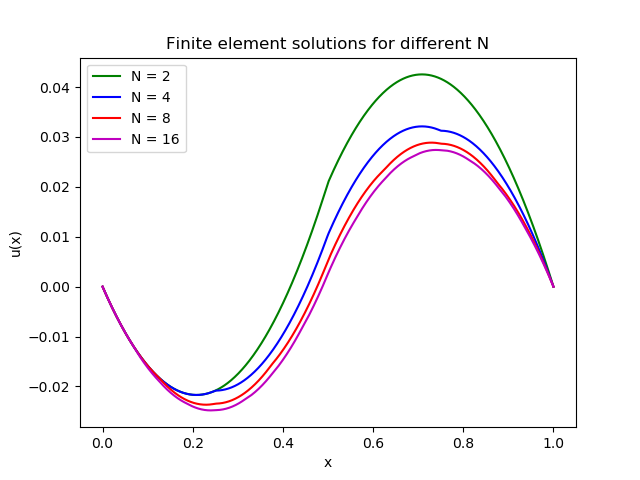
\includegraphics[width=5in]{soln.png}
\end{figure}


%%%%%%%%%%%%%%%%%%%%%%%%%%%%%%%%%%%%%%%%%%%%%%%%%%%%%

  \end{enumerate}

\end{enumerate}




\end{document}
